\section{The lattice-Boltzmann method}

\subsection{Introduction}

\begin{frame}{Historical overview}

\begin{itemize*}

\item Lattice gas automata (LGA) methods 70's, 80's

\begin{figure}
  \centering
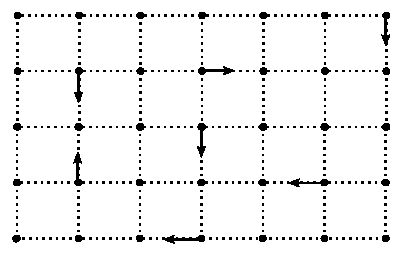
\includegraphics[width=0.6\textwidth]{../fig/lga.pdf}
\end{figure}

\item Several flaws of the LGA cured: continuous distributions, higher
  symmetry in lattices... $\implies$ LBM late 80's, 90's, 00's

\end{itemize*}

\end{frame}

\subsection{Basic idea}


\begin{frame}{Basic idea}

\begin{itemize*}

\item Discretisation of phase space $\implies$ the lattice, example D2Q9:
\begin{figure}
  \centering
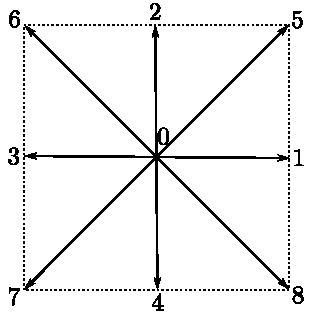
\includegraphics[width=0.35\textwidth]{../fig/lattice_d2q9.pdf}
\end{figure}

\item The distribution function $\fii(\x, t)$ - probability of finding
  a particle at $\x$, t with velocity $\ci$.
\end{itemize*}


\end{frame}

\begin{frame}{Basic idea}

\begin{itemize*}
\item Evolution of $\fii$, the lattice-Boltzmann equation:

\begin{equation}\label{eq:lbm:lbe}
f_i(\x + \cbf_i\delta_t, t + \delta_t) - f_i(\x, t) = \Omega_{ij}(\x, t)
\end{equation}

\item A popular choice is the BGK collision operator:

\begin{equation}\label{eq:lbm:bgk}
\Omega_{ij} = \Omega_i = -\omega \left[ f_i(\x, t) - f_i^{(eq)}(\x, t)
  \right]
\end{equation}

\end{itemize*}

\end{frame}

\begin{frame}{Basic idea}
In the case with Navier-Stokes we have:

\begin{equation}\label{eq:lbm:ns_eq}
\feq = w_i\rho \left [ 1 + \frac{\ci \cdot \ubf}{c_s^2} +
  \frac{(\ci \cdot \ubf)^2}{2c_s^4} - \frac{\ubf^2}{2c_s^2} \right]
\end{equation}

The macroscopic quantities $\rhorm$ and $\ubf$ are obtained from
$\fii$ through:

\begin{equation}\label{eq:lbm:rho_mom}
\rhorm = \sum_i \fii
\end{equation}
and
\begin{equation}\label{eq:lbm:j_mom}
\rhorm \ubf = \sum_i \fii \ci .
\end{equation}

\end{frame}

\begin{frame}{Coupled scheme}
\begin{figure}
\begin{center}
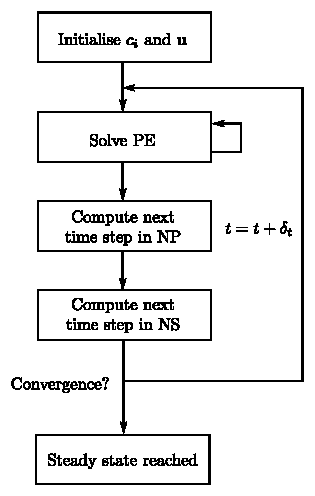
\includegraphics[width=0.4\textwidth]{../fig/full_algorithm.pdf}
\end{center}
\end{figure}
\end{frame}

\subsection{Boundary conditions}

\begin{frame}[t]{Boundary conditions}

\begin{itemize*}
\item[] \begin{figure}
\begin{center}
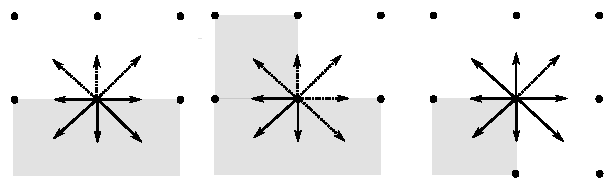
\includegraphics[width=0.9\textwidth]{../fig/bb.pdf}
\end{center}
\end{figure}

\item Bounce back ($\ubf = 0$)

\item Mirror reflection ($\J_{ion} \cdot \mathbf{n} = 0$ and $\nabla\psirm
  \cdot \n = -\sigma_s/\epsilon_0\epsilon_r$)

\end{itemize*}

\begin{figure}
  \subfloat{\label{fig:lbm:no_slip}\includegraphics<2->[width=0.35\textwidth]{../fig/no_slip.pdf}}
  \hspace{5pt}
  \subfloat{\label{fig:lbm:slip}\includegraphics<3>[width=0.35\textwidth]{../fig/slip.pdf}}
\end{figure}

\end{frame}

%\subsection{How}
